\documentclass[10pt]{report}

\usepackage{amssymb}
\usepackage{amsthm}
\usepackage{amsmath}
\usepackage{amstext}
\usepackage[utf8]{inputenc}
\usepackage{graphicx}
\usepackage{makeidx}
\usepackage{caption}
\usepackage{float}
\usepackage{verbatim}
\usepackage{epigraph}
\usepackage[italian]{babel}
\usepackage[margin=1in]{geometry}
\usepackage{titlesec}
\usepackage{xcolor}
\usepackage{enumitem}
\usepackage[htt]{hyphenat}
\usepackage{tikz}
\usepackage{verbatim}
\usepackage{metalogo}


\usetikzlibrary{mindmap, trees}



% Titles stuff: %
\titleformat{\chapter}[display]
{\normalfont\huge\bfseries}{}{0pt}{\Huge}
\titleformat{\section}[display]
{\normalfont\Large\bfseries}{}{0pt}{\Large}
\titleformat{\subsection}[display]
{\normalfont\large\bfseries}{}{0pt}{\large}
\titleformat{\subsubsection}[display]
{\normalfont\normalsize\bfseries}{}{0pt}{\normalsize}

% Math-set Stuff: %
\newcommand{\mb}{\mathbb}
\newcommand{\R}{\mb R}
\newcommand{\N}{\mb N}
\newcommand{\C}{\mb C}

%\author{Carlo Buccisano}
%\title{I Frattali}
%\date{Anno scolastico 2015-2016}


% Prevent from breaking lines and formulas: %
%\hyphenpenalty 10000
%\exhyphenpenalty 10000
\relpenalty=10000
\binoppenalty=10000


\begin{document}
	\begin{titlepage}
		\begin{minipage}{0.3\textwidth}
			
\includegraphics[width=0.3\textwidth]{Copertina/logo}
		\end{minipage}
		\hfill
		\begin{minipage}{0.6\textwidth}\raggedleft
			Liceo Scientifico Lussana\\
			Tesina Esame di Stato\\
			Anno scolastico 2015-2016
		\end{minipage}
		\centering
		\vspace*{\stretch{1}}
		\begin{center}
			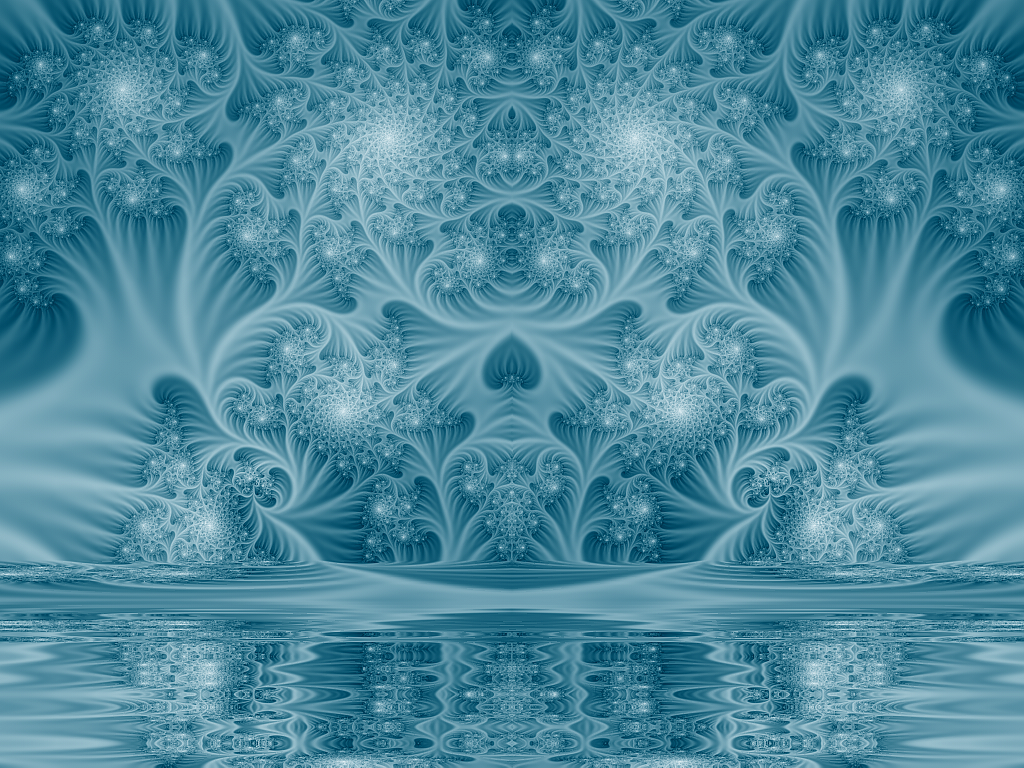
\includegraphics[width=1\linewidth]{Copertina/blue_lagoon}
		\end{center}
		\vspace*{\stretch{1}}
		{\Large Carlo Buccisano\par}
		\vspace{1cm}
		\textcolor{red}{\Huge{I Frattali}}
		\par
	\end{titlepage}
	%\maketitle
	
	\begin{comment}
		\chapter{Introduzione}
			\section{Trasformazione geometrica}
				Una \textbf{trasformazione geometrica} $T$  è una corrispondenza biunivoca che a ogni punto $P$ di un piano associa uno e un solo punto $P'$ appartenente ad un altro piano (eventualmente anche lo stesso di partenza).\\
				Fissato un sistema cartesiano $Oxy$ la coordinate del punto $P'(x', y')$ possono essere espresse in funzione di quelle del punto $P(x, y)$:\\\\
				$
				\begin{cases}
					x' = f(x, y)\\
					y' = g(x, y)\\
					
				\end{cases}
				$\\\\\\
				dove $f$ e $g$ sono due funzioni ovunque definite e invertibili. 
				
			\section{Affinità}
				Un'affinità tra due piani $\pi$ e $\pi'$ è una trasformazione geometrica $T$ che fa corrispondere al punto $P(x, y) \in \pi$ il punto $P'(x', y') \in \pi'$ tale che:\\\\
				$\begin{cases}
				x' = ax + by + e\\
				y' = cx + dy + f
				\end{cases}$\\\\\\
				dove $a, b, c, d, e, f \in \R$.\\\\\\
				Usando il prodotto tra matrici l'affinità può essere definita anche come:\\\\
				$ \left( \begin{array}{c}x'\\y' \end{array}\right) =  \left( \begin{array}{cc}a & b\\c & d\end{array} \right) \cdot \left( \begin{array}{c}x\\y\end{array}\right) + \left( \begin{array}{c}e\\f\end{array}\right)$\\
				dove la matrice caratteristica è $A = \left( \begin{array}{cc}a & b\\c & d\end{array} \right)$ tale che $det(A) = ab - bc \neq 0$.
				
				\subsection*{Proprietà fondamentali}
				Si dimostra che l'affinità gode delle seguenti proprietà:\\
				\begin{itemize}
					\item trasforma rette in rette;
					\item il parallelismo è un'invariante dell'affinità (ovvero rette parallele e incidenti rimangono tali);
					\item il rapporto tra segmenti paralleli è conservato (ad esempio al punto medio di un segmento corrisponde il punto medio del segmento trasformato);
					\item una figura $B$ di area $S$ viene mandata in una figura $B'$ di area $S' = det(A) \cdot S$, dove $A$ è la matrice caratteristica.				
				\end{itemize}
				In generale comunque l'affinità non conserva la forma degli oggetti: l'affine di una circonferenza è un'ellisse e di un rettangolo è un parallelogramma.
				
				\subsection*{Punti uniti}
				Se il piano iniziale e finale coincidono, si possono avere elementi che hanno come immagine se stessi, i cosiddetti punti uniti.\\
				Per trovarli basta risolvere il sistema:\\\\
				$\begin{cases}
				x = ax + by + e\\
				y = cx + dy + f
				\end{cases}$\\\\\\
				il quale potrà avere una sola soluzione, infinite soluzioni (infiniti punti, tutti appartenenti alla stessa retta) oppure nessuna soluzione.
				
				\subsection*{Tipi particolari}
				Le affinità possono essere classificate a seconda dei loro invarianti, ovvero le proprietà delle figure che restano inalterate nelle loro trasformate.\\
				Se l'ampiezza degli angoli rimane invariata, l'affinità è detta \textit{similitudine}.\\
				Se anche le distanze e le aree vengono conservate, l'affinità è detta \textit{isometria} (particolare tipo di similitudine).\\
				Infine componendo due o più affinità si ottiene sempre un'affinità.
	\end{comment}
	
	% Mappa concettuale: %
	\begin{comment}
		\begin{tikzpicture}
		\path[mindmap,concept color=black,text=white]
		node[concept] {I Frattali}
		[clockwise from=0]
		child[concept color=green!50!black] {
			node[concept] {Cos'è un frattale}
			[clockwise from=90]
			child { node[concept] {Dimensione non intera} }
			child { node[concept] {Tipi di frattali} }
			child { node[concept] {Frattali in natura} }
			child { node[concept] {Applicazioni pratiche} }
		}  
		child[concept color=blue] {
			node[concept] {Frattali famosi}
			[clockwise from=-30]
			child { node[concept] {Insieme di Mandelbrot} }
			child { node[concept] {Insieme di Julia} }
			child { node[concept] {Insieme di Cantor} }
		}
		child[concept color=red] { node[concept] {James Joyce} 
			[clockwise from=-70]
			child { node[concept] {Ulysses} }
			child { node[concept] {Finnegans Wake} }
			child { node[concept] {Multifractal Structure of Finnegans Wake} }
		}
		child[concept color=orange] { node[concept] {Eterno Ritorno dell'uguale} };
		\end{tikzpicture}
		\newpage
	\end{comment}
	\begin{tikzpicture}
	\path [
		mindmap,
		text = white,
		level 1 concept/.append style =
		{font=\Large\bfseries, sibling angle=90},
		level 2 concept/.append style =
		{font=\normalsize\bfseries},
		level 3 concept/.append style =
		{font=\small\bfseries},
		tex/.style     = {concept, ball color=blue, font=\Huge\bfseries},
		engines/.style = {concept, ball color=green!50!black},
		formats/.style = {concept, ball color=blue!50!black},
		systems/.style = {concept, ball color=red!90!black},
		editors/.style = {concept, ball color=orange!90!black}
	]
	node [tex] {I Frattali} [clockwise from=0]
		child[concept color=green!50!black, nodes={engines}] {
			node {Cos'è un frattale} [clockwise from=90]
				child { node {Dimensione non intera} }
				child { node {Tipi di frattali} }
				child { node {Frattali in natura} }
				child { node {Applicazioni pratiche} }
		}
		child [concept color=blue, nodes={formats}] {
			node {Frattali famosi} [clockwise from=325]
				child { node {Insieme di Cantor} }
				child { node {Insieme di Mandelbrot} }
				child { node {Insieme di Julia} }
		}
		child [concept color=red, nodes={systems}] {
			node {James Joyce} [clockwise from=210]
			child { node {Ulysses} } 
			child { node {Finnegans Wake}  [clockwise from=60]
				child { node {Fractal structure}}
			}
		}
		child [concept color=orange, nodes={editors}] {
			node {Eterno ritorno dell'uguale} 
		};
	\end{tikzpicture}
	\newpage
	
	\tableofcontents
	\newpage
	\chapter{Premessa}
		Fin da piccolo sono stato appassionato alla matematica e all'informatica, passioni poi consolidatesi al liceo grazie anche ad iniziative come le Olimpiadi di Informatica e di Matematica.\\ Circa un anno fa ho scoperto, sentendone parlare da un amico, il mondo dei frattali e di come si potessero generare al computer, e da subito mi sono appassionato e ho provato a scrivere io stesso dei programmi per generarli. Ho così scoperto una branca della matematica, relativamente recente, che reputo molto interessante e che, oltre ad essere rilevante dal punto di vista matematico, presenta anche diverse applicazioni pratiche, come lo studio delle coste o dei sistemi dinamici, e può essere ``apprezzata'' anche dai non-esperti grazie alle suggestive immagini dei frattali più famosi. Inoltre ho trovato nella geometria frattale un collegamento tra le discipline che amo di più: matematica per la teoria e informatica per quanto riguarda la generazione delle immagini.\\ Con questa tesina ho voluto studiare i principali frattali, oltre che alcuni dei più comuni algoritmi per generarli.
	\chapter{I Frattali}
		\epigraph{``Why is geometry often described as ``cold'' and ``dry''? One reason lies in its inability to describe the shape of a cloud, a mountain, a coastiline, or a tree. Clouds are not spheres, mountains are not cones, coastlines are not circles, and bark is not smooth, nor does lightning travel in a straight line.''}{\textit{The Fractal Geometry Of Nature}, Benoît B. Mandelbrot}
		\section{Cos'è un frattale}
			Gli oggetti naturali (alberi, montagne, nuvole, felci...) spesso non possono essere studiati usando la geometria euclidea, a causa del loro carattere fortemente irregolare. Ciò ha giustificato l'introduzione di un nuovo tipo di geometria nel 1982 da parte del matematico Benoît B. Mandelbrot (1924 - 2010): la geometria frattale.\\
			In realtà già in passato alcuni frattali erano noti (basti pensare ai tanti descritti da Cantor, Peano, Sierpinski, Koch...) ma erano considerati ``curve patologiche'', ``mostri matematici'' e solo grazie a Mandelbrot essi vennero formalizzati e approfonditi.\\
			Il concetto di frattale appare per la prima volta nel libro \textit{The Fractal Geometry of Nature}, pubblicato nel 1983 da Mandelbrot. La definizione più semplice di frattale è quella di  figura geometrica caratterizzata dal ripetersi all'infinito di uno stesso motivo, su scala sempre più ridotta, proprietà detta autosimilarità. Ciò significa che ingrandendo la figura si troveranno forme ricorrenti e che ad ogni ingrandimento essa si arricchirà di nuovi particolari.\\
			Il termine frattale è un neologismo introdotto dallo stesso Mandelbrot e deriva dal latino ``fractus'', cioé rotto.\\
			Un frattale, per poter essere definito tale, deve possedere alcune caratteristiche tra cui:
			\begin{itemize}
				\item \textbf{autosimilarità}: in geometria due poligoni sono detti simili se e solo se hanno angoli uguali e lati in proporzione. Per i frattali l'autosimilarità consiste nel fatto che una loro parte è simile al frattale di partenza.
				\item \textbf{perimetro infinito o nullo}: spesso i frattali hanno perimetro infinito e area finita, proprietà riscontrabile anche nella realtà, per elementi con contorni molto irregolari. Un esempio classico, che Mandelbrot studiò, è il profilo delle coste. 
				\item \textbf{area finita o nulla}: nonostante i frattali possano avere perimetro infinito, la loro area sarà sempre finita o nulla.
				\item \textbf{irregolarità}: un frattale non può essere definito come luogo di punti che soddisfino certe condizioni geometriche o analitiche, perché per descriverlo si utilizzano definizioni ricorsive (dunque il frattale è generato con un algoritmo e non con un'equazione).
			\end{itemize}
			
		\section{Principali tipi di frattali}
			I frattali possono essere classificati secondo differenti criteri.\\
			Ad esempio secondo la classificazione fisico-geometrica si distinguono i frattali biomorfi (che rappresentano oggetti verosimili) da quelli decorativi. Si distinguono poi i frattali \textit{deterministici}, che vengono costruiti sempre nel medesimo modo con le stesse trasformazioni/formule, e quelli \textit{aleatori} o non deterministici, durante la costruzione dei quali intervengono anche parametri casuali, che quindi possono variare di volta in volta, importantissimi nello studio dei sistemi dinamici caotici come la turbolenza.
			Infine si possono distinguere i frattali in base ai metodi di costruzione al calcolatore, i cui principali sono elencati di seguito.
			\subsection{Frattale IFS}
				Alcuni tipi di frattali, i frattali IFS (\textit{Iterated Function System}), possono essere definiti tramite sequenze di trasformazioni geometriche: si consideri un insieme di $N$ trasformazioni del piano cartesiano $\{T_1, ...,T_{N}\}$ e un sottoinsieme iniziale $A$ di punti del piano. Applicando ogni trasformazione ad esso si otterranno altri $N$ sottoinsiemi di punti del piano $\{T_1(A), ...,T_N(A)\}$, la cui unione costituirà un altro nuovo sottoinsieme $A_1$. Continuando così si otterranno gli insiemi $A_2, A_3...$ e così via.\\
				Se la successione di insiemi \textit{converge} ad un insieme limite $F$ (ovvero si stabilizza, da un certo punto in poi non vi sono più cambiamenti apprezzabili) allora $F$ è definito frattale IFS.\\
				Un'interessante proprietà è che, cambiando l'insieme di partenza ma mantendendo le stesse trasformazioni geometriche, il risultato finale non cambia, cioé il frattale ottenuto dipende solamente dalle trasformazioni e non dall'insieme di partenza.
			
			\subsection{Frattale LS}
				Un'altra classe di frattali è quella dei frattali LS (\textit{Lindenmayer-System}, dal nome dello studioso che negli anni '60 li ha introdotti per studiare i fenomeni di crescita delle piante), che possono essere visti come una generazione dei frattali IFS (tutti i frattali IFS sono anche LS, ma non vale il viceversa).\\
				Un frattale LS non è propriamente autosimile, in quanto non è possibile suddividere la figura in un certo numero di parti simili ad essa. \`E però possibile suddividere il frattale in un numero \emph{finito} di frattali IFS.\\
				Il metodo di Lindenmayer per generare frattali (non solo LS) è completamente diverso dalle trasformazioni geometriche usate negli IFS: si immagina di avere un cursore che può avanzare e lasciare una traccia sul piano. Più precisamente questo cursore è soggetto a delle regole ben precise:
				\begin{itemize}
					\item Regola \textbf{F}: avanzare di un segmento di lunghezza fissata
					\item Regola \textbf{f}: avanzare di un segmento di lunghezza fissata, ma senza lasciare traccia
					\item Regola \textbf{+}: ruotare in senso antiorario di un angolo assegnato
					\item Regola \textbf{-}: ruotare in senso orario di un angolo assegnato
				\end{itemize}
				Si parte da una costruzione iniziale, detta \textit{assioma}, e si effettua ogni volta una sostituzione secondo una regola assegnata e iterando infinite volte il procedimento si ottiene il frattale desiderato. Un esempio interessante di tale procedimento è la curva di Koch.
			\subsection{Frattale basato su una formula}
				Per generare questi frattali si utilizza una funzione generatrice (reale o complessa) da iterare per ogni punto (pixel) del frattale. Spesso, come ad esempio nell'insieme di Mandelbrot, per ogni punto si controlla se la successione ottenuta dall'iterazione della funzione scelta diverga o no. In base al tipo di funzione di partenza si distinguono:
				\begin{itemize}
					\item \textbf{Frattali lineari}: frattali la cui funzione generatrice contiene solo termini del primo ordine
					\item \textbf{Frattali non lineari}: frattali la cui funzione generatrice contiene termini di ordine superiore al primo, ad esempio la celebre funzione complessa $f_c(z) = z^2 + c$ studiata nel 1918 da Gaston Julia e poi divenuta celebre grazie all'insieme di Mandelbrot.
				\end{itemize}

		\section{Dimensione non intera}
			Il concetto di dimensione classico della topologia, già presente implicitamente in Euclide, è stato inizialmente definito da Poincaré. Secondo questa definizione a un punto, o a un insieme totalmente sconnesso di punti, è assegnata dimensione $D_{\tau} = 0$, e in generale, dato un oggetto $F$, la sua dimensione topologica $D_{\tau}$ è il numero tale che, preso un intorno arbitrariamente piccolo di un punto di $F$, la sua frontiera ha dimensione $D'_{\tau} = D_{\tau} - 1$.\\
			Ad esempio, se si considera una retta, essa ha dimensione $1$ in quanto la frontiera di ogni suo intorno ha dimensione $0$. In generale si può capire come questa definizione assegni solamente numeri interi come dimensioni.\\\\
			Il concetto di dimensione topologica di Poincaré, però, non è esaustivo per descrivere i frattali e da ciò deriva l'ampliamento del concetto di dimensione per i frattali, la cosiddetta \textit{dimensione di Hausdorff}.\\
			Per definire la dimensione frattale ci si riferisce alla proprietà di autosimilarità, che hanno anche quadrati o cubi. Essa afferma che l'oggetto considerato può essere diviso in un certo numero $N$ di parti simili all'oggetto intero: ad esempio ogni segmento può essere diviso in $N$ parti ognuna lunghe $\frac{1}{N}$, così come il cubo di volume unitario può essere diviso in $N^3$ cubetti ognuno avente volume $\frac{1}{N^3}$. 
			In tali casi l'esponente di $N$ corrisponde alla dimensione topologica e generalizzando si può affermare che se $K$ è il rapporto dell'omotetia per ottenere, dall'oggetto iniziale, una delle parti allora:\\
			\begin{gather*}
				D_f = \frac{\log N}{\log ( 1 / K )}
			\end{gather*}
			\\\\
			La dimensione di un frattale così definita non è intera e si può affermare che un frattale è tale se ha dimensione frattale $D_f$ maggiore della sua dimensione topologica $D_{\tau}$.\\\\
			\begin{footnotesize}
				N.B.: la base del logaritmo nella formula è indifferente dal momento che si considera un rapporto tra logaritmi.
			\end{footnotesize}
		\newpage
		\section{Frattali in natura}
			In natura si trovano moltissimi esempi di oggetti il cui schema sembra essere molto più aderente alla geometria frattale rispetto a quella euclidea. Basti pensare al profilo frastagliato delle foglie, degli alberi, alle diramazioni dei dendriti nervosi o ai fulmini.\\
			Alcuni dei più comuni frattali biomorfi:\\
			\begin{figure}[H]
				\minipage{0.5\textwidth}
				\centering
				\includegraphics[width=0.7\linewidth]{"Frattali in natura/Fractal_Broccoli"}
				\caption*{Broccolo romanesco}
				\label{fig:broccolo}
				\endminipage \hfill
				\minipage{0.5\textwidth}
				\centering
				\includegraphics[width=0.7\linewidth]{"Frattali in natura/ammoniti"}
				\caption*{Ammoniti}
				\label{fig:ammoniti}
				\endminipage \hfill
			\end{figure}
			\begin{figure}[H]
				\minipage{0.5\textwidth}
				\centering
				\includegraphics[width=0.7\linewidth]{"Frattali in natura/albero-frattale"}
				\caption*{Struttura frattale albero}
				\label{fig:albero}
				\endminipage \hfill
				\minipage{0.5\textwidth}
				\centering
				\includegraphics[width=0.7\linewidth]{"Frattali in natura/intense-fulminazioni"}
				\caption*{Fulmini}
				\label{fig:fulmine}
				\endminipage \hfill
			\end{figure}
			\begin{figure}[H]
				\minipage{0.5\textwidth}
				\centering
				\includegraphics[width=0.3\linewidth, height=0.2\textheight]{"Frattali in natura/felcebarnsley"}
				
				\caption*{Struttura frattale felce}
				\label{fig:felce}
				\endminipage \hfill
				\minipage{0.5\textwidth}
				\centering
				\includegraphics[width=0.7\linewidth]{"Frattali in natura/paesaggio_frattale"}
				\caption*{Paesaggio frattale}
				\label{fig:paesaggio}
				\endminipage \hfill
			\end{figure}

		\section{Applicazioni dei frattali}
			Al giorno d'oggi i frattali trovano numerose applicazioni: ad esempio vengono usati da ingegneri e fisici per creare modelli che descrivono il moto di fluidi turbolenti o fenomeni di combustione. Un'altra importante branca dove vengono utilizzati è la compressione di video e immagini, sfruttando le proprietà di autosimilarità del file da comprimere. Inoltre i frattali vengono impiegati anche per lo studio della natura: dalle linee di costa, ai corsi dei fiumi e alle catene montuose. La percolazione, il lento movimento di un fluido su un materiale poroso, è studiato tramite modelli frattali.
	\chapter{Frattali famosi}
		\section{Curva di Koch}
			La curva (o merletto) di Koch deve il suo nome al matematico H. Von Koch (1870 - 1924) che nel 1904 introdusse questa ``curiosa'' curva, molto tempo prima che venisse introdotto il concetto di frattale.\\
			Essa, come tutti i frattali, è costruita tramite un algoritmo ricorsivo, a partire da un segmento di lunghezza unitaria:
			\begin{enumerate}
				\item si divide il segmento in 3 parti uguali
				\item si cancella la parte centrale e la si sostituisce con 2 segmenti uguali ad essa che formino i lati di un triangolo equilatero
				\item si riparte col punto 1 per ogni segmento ottenuto
			\end{enumerate}
			
			\begin{center}
				\includegraphics[width=0.2\linewidth, height=0.2\textheight]{"Curva di Koch/koch"}
			\end{center}
			
			\bigskip
			\bigskip
			Dalla figura è evidente la proprietà di autosimilarità: infatti la curva, indipendentemente dall'ingrandimento, può essere divisa in quattro parti simili al frattale iniziale.
			\begin{center}
				\includegraphics[width=0.4\linewidth, height=0.1\textheight]{"Curva di Koch/kochcolori"}
			\end{center}
			
			La curva di Koch può essere divisa in $N = 4$ parti con rapporto di omotetia $K = 1/3$ rispetto all'iniziale frattale dunque la dimensione frattale della curva è:
			\begin{gather*}
				D_f = \frac{\log 4}{\log 3} \approx 1.2619
			\end{gather*}
			mentre la dimensione topologica è $D_{\tau} = 1$.\\
			La curva può essere generata tramite il metodo LS: l'assioma iniziale è \textbf{F} (un segmento), l'angolo è di $60$ gradi e ad ogni iterazione si sostituisce ad ogni \textbf{F} la stringa \textbf {F+F-F+F} (segmento con la parte centrale modificata).
		\section{Fiocco di Koch}
			Un frattale LS è il fiocco di Koch, detto anche fiocco di neve. Esso può essere ottenuto combinando insieme tre copie della curva di Koch lungo i lati di un triangolo equilatero. Più precisamente si ottiene applicando lo stesso algoritmo della curva di Koch, partendo però non da un singolo segmento ma da un triangolo equilatero.\\
			Esso non è propriamente autosimile: non è infatti possibile suddividerlo in parti simili alla figura iniziale, ma è possibile dividerlo in un numero finito di curve di Koch, frattali IFS, e dunque esso appartiene alla classe dei frattali LS.
			\begin{center}
				\includegraphics[width=0.3\linewidth, height=0.2\textheight]{"Fiocco di Koch/fioccodineve"}
			\end{center}
			Si può dimostrare facilmente che il perimetro del fiocco è infinito. 
			Sia $p_0 > 0$ il perimetro iniziale del triangolo e $p_n$ il perimetro della figura all'n-esima iterazione dell'algoritmo, il perimetro finale $p$ sarà:
			\begin{gather*}
				p = \lim_{n \rightarrow + \infty} p_n
			\end{gather*}
			Considerando un singolo segmento, ad ogni iterazione la sua lunghezza viene moltiplicata per $4 / 3$, dunque, sommando la lunghezza di tutti i segmenti si ottiene il perimetro della figura e, raccogliendo a fattore comune $4/3$ si ricava che:
			\begin{gather*}
				p_n = \left( \frac{4}{3} \right)^n \cdot p_0
			\end{gather*}
			da cui:
			\begin{gather*}
				p = \lim_{n \rightarrow + \infty} p_n = \lim_{n \rightarrow + \infty} \left(\frac{4}{3} \right)^n \cdot p_0 = + \infty
			\end{gather*}
			
			Nonostante abbia un perimetro infinito, il fiocco di Koch ha area finita. \\\\
			Infatti sia $A_0 > 0$ l'area del triangolo iniziale e $N_0 = 3$ il numero di lati iniziali della figura. Ad ogni iterazione, ogni lato dà origine a 4 nuovi lati, dunque all'$n$-esima iterazione vi sono $N_n = 4^n \cdot N_0$ lati. \\Inoltre, in tale iterazione, i triangoli aggiunti, tanti quanti i lati della figura nell'iterazione precedente ($N_{n-1}$), hanno tutti area pari a $1/9$ dell'area dei triangoli precedenti ($A_{n-1}$), da cui si ricava facilmente che la loro area vale $A_n = \left( \frac{1}{9} \right) ^ n \cdot A_0$.\\
			Dunque detta $S_n$ l'area totale del fiocco all'$n$-esima iterazione vale:
			\begin{gather*}
				S_n = A_0 + \sum_{i=1}^{n} N_{i-1} \cdot A_{i} = 
		        A_0 + \sum_{i=1}^{n} 4^{i-1} \cdot N_0 \cdot \left( \frac{1}{9} \right) ^ i \cdot A_0 =
		        A_0 \cdot \left( 1 + N_0 \cdot \sum_{i=1}^{n} 4^{i-1} \cdot \left( \frac{1}{9} \right) ^ i  \right)
			\end{gather*}
			e sostituendo i dati numerici:
			\begin{gather*}
				S_n = A_0 \cdot \left( 1 + \frac{1}{3} \cdot \sum_{i=0}^{n-1} \left(\frac{4}{9}\right)^i \right) 
			\end{gather*} 
		
			L'area finale del frattale sarà quindi uguale a:
			\begin{gather*}
				S = \lim_{n \to +\infty} S_n = \lim_{n \to +\infty} A_0 \cdot \left( 1 + \frac{1}{3} \cdot \sum_{i=0}^{n-1} \left(\frac{4}{9}\right)^i \right) = \lim_{n \to +\infty} A_0 \cdot \left(1 + \frac{1}{3} \cdot \frac{ \left( \frac{4}{9} \right) ^ n - 1}{\frac{4}{9} - 1} \right) \\
				= A_0 \cdot \left(1 + \frac{1}{3} \cdot \frac{1}{1 - \frac{4}{9}} \right) = \frac{8}{5} \cdot A_0
			\end{gather*}
			\begin{footnotesize}
				N.B.: il perimetro della figura inteso in senso ``tradizionale'' è infinito, però ciò non è propriamente vero in quanto la curva ha dimensione $\frac{\log 4}{\log 3}$, non permettendo di definire la misura del perimetro una vera e propria lunghezza.
			\end{footnotesize}
		
		\section{Insieme di Cantor}
			L'insieme di Cantor, introdotto dal matematico tedesco Georg Cantor (1845 - 1918), è un sottoinsieme dell'intervallo $[0, 1]$ dei numeri reali.\\
			Esso è un frattale IFS in quanto ha la classica proprietà di autosimilarità e può essere costruito col seguente algoritmo ricorsivo:
			\begin{enumerate}
				\item si divide l'intervallo in tre parti congruenti
				\item si rimuove il segmento centrale aperto (dunque i due estremi non vengono rimossi), ottenendo così due intervalli (chiusi) più piccoli
				\item si riapplica il punto 1. ai due intervalli ottenuti
			\end{enumerate}
			\begin{center}
				\includegraphics[width=0.7\linewidth]{"Insieme di Cantor/cantor_set_in_seven_iterations"}
			\end{center}
			L'insieme di Cantor contiene tutti i punti che non vengono mai rimossi dall'intervallo iniziale applicando infinite volte la procedura sopra descritta e, per questo, è talvolta anche chiamato \textit{polvere di Cantor}.\\
			Ad ogni passo viene rimosso un terzo del numero di punti (ogni intervallo diventa i $2/3$ del precedente) dunque il perimetro finale del frattale è:
			\begin{gather*}
				p = \lim_{n \to +\infty} \left( \frac{2}{3} \right) ^ n \cdot 1 = 0
			\end{gather*}
			Nonostante il perimetro dell'insieme sia nullo, l'insieme di Cantor non è vuoto: infatti se ad una certa iterazione $n$ dell'algoritmo si arriva ad un intervallo continuo $[a, b] \in [0, 1]$ allora le successive iterazioni non rimuoveranno mai dall'insieme i punti $a$ e $b$.\\
			Vi sono poi altri punti che appartengono all'insieme di Cantor senza mai essere estremi di intervalli, come ad esempio $1/4 = 020202..._3$, come si noterà in seguito.\\
			Si può inoltre dimostrare che l'insieme contiene tanti punti quanti ne contiene l'intervallo $[0, 1]$, entrambi aventi la cardinalità del continuo.
			Se si considera la rappresentazione in base $3$ dei reali tra $0$ e $1$ si nota che $1/3 = 0.1_3$ e che $2/3 = 0.2_3$, quindi nella prima iterazione in cui vengono rimossi tutti i punti $t$ tali che $1/3 < t < 2/3$, vengono rimossi tutti quei numeri la cui scrittura in base $3$ è della forma $0.1xxx.._3$, dove $xxx..._3$ è una qualsiasi sequenza di $0, 1, 2$ diversa da $000..._3$ e da $222..._3$.\\
			Dopo la prima iterazione rimangono quindi solo i numeri che in base $3$ sono scrivibili come $0.0xxx..._3$ o $0.2xxx..._3$ (ricordandosi che $1/3 = 0.1_3 = 0.0222..._3$ e che $2/3 = 0.1222..._3 = 0.2_3$). Per le iterazioni successive si dimostra allo stesso modo che all'$n$-esima iterazione tutti i numeri aventi come $n$-esima cifra decimale $1$ nella loro rappresentazione in base $3$ vengono rimossi.\\
			Dunque alla fine nell'insieme rimangono solamente tutti i reali scrivibili come $0.xxx_3$, usando solo le cifre $0$ e $2$. \\
			Ora se si considera la funzione $f: \mbox{Insieme di Cantor} \to [0, 1]$ che associa ad ogni numero dell'insieme il numero binario (in base $2$) che si ottiene sostituendo la cifra $1$ a $2$, si nota che si ottengono tutti i reali dell'intervallo $[0, 1]$.
			La funzione $f$ è suriettiva dal momento che ogni numero dell'intervallo $[0, 1]$ in binario viene scritto come $0.yyy..._2$ dove $y$ è 0 o 1 ed è anche iniettiva dato che ad ogni numero dell'insieme di Cantor corrisponde uno e un solo numero binario tra $0$ e $1$.\\
			Essendo $f$ sia suriettiva sia iniettiva, $f$ è una funzione biunivoca che dimostra che l'insieme di Cantor e l'intervallo $[0, 1]$ hanno la stessa cardinalità, ovvero la cardinalità del continuo, $\mathfrak{c} = 2^{\aleph_0}$.\\
			L'insieme di Cantor, ad ogni iterazione, viene diviso in due parti simili al frattale stesso, con fattore di omotetia $K=1/3$ dunque la sua dimensione di Hausdorff è:
			\begin{gather*}
				D_f = \frac{\log 2}{\log 3} \approx 0.6309
			\end{gather*}
			Esistono anche rappresentazioni bidimensionali e tridimensionali dell'insieme di Cantor, ottenute applicando lo stesso algoritmo a partire, rispettivamente, da un quadrato e da un cubo.
			
			\begin{figure}[H]
				\minipage{0.5\textwidth}
					\centering
					\includegraphics[width=0.4\linewidth]{"Insieme di Cantor/Cantor_dust"}
					\caption*{Polvere di Cantor 2D}
					\label{fig:cantor2d}
				\endminipage \hfill
				\minipage{0.5\textwidth}
					\centering
					\includegraphics[width=0.4\linewidth]{"Insieme di Cantor/3D_Cantor_set"}
					\caption*{Polvere di Cantor 3D}
					\label{fig:cantor3d}
				\endminipage
			\end{figure}
		\section{Triangolo di Sierpiński}
			Il triangolo di Sierpinski è un frattale IFS, così chiamato dal nome di Wacław Sierpiński (1882 - 1969), che lo descrisse nel 1915.\\
			L'algoritmo che permette di ottenerlo a partire da un triangolo è il seguente:
			\begin{enumerate}
				\item si uniscono i punti medi del triangolo, dividendolo in altri quattro triangoli congruenti
				\item si rimuove il triangolo centrale
				\item si riparte dal punto 1. per tutti i triangoli
			\end{enumerate}
			
			\begin{center}
				\includegraphics[width=0.3\linewidth]{"Triangolo di Sierpinski/SierpinskiTriangle"}
			\end{center}

			Il frattale può essere diviso in $N = 3$ figure simili a quella iniziale, con rapporto di similitudine $K = 1/2$ dunque la sua dimensione di Hausdorff è:
			\begin{gather*}
				D_f = \frac{\log 3}{\log 2} \approx 1.585
			\end{gather*}
			Inoltre il triangolo di Sierpiński ha area nulla: infatti se $A_0$ è l'area iniziale, ad ogni iterazione l'area diventa i $3/4$ della precedente, quindi all'$n$-esima iterazione l'area diventa $A_n = \left( \frac{3}{4} \right) ^ n \cdot A_0$, da cui si ricava che l'area finale è:
			\begin{gather*}
				A = \lim_{n \to + \infty} A_n = \lim_{n \to +\infty} \left( \frac{3}{4} \right)^n \cdot A_0 = 0
			\end{gather*}
			
		\section{Tappeto di Sierpiński}
			Il tappeto di Sierpiński è un frattale simile all'insieme di Cantor ottenuto a partire da un quadrato, descritto dal matematico polacco Wacław Sierpiński nel 1916.\\
			Esso è molto simile al triangolo di Sierpiński. L'algoritmo che, a partire da un quadrato, permette di generarlo è il seguente:
			\begin{enumerate}
				\item si divide il quadrato in 9 quadrati congruenti più piccoli
				\item si rimuove il quadrato centrale (solo la parte interna)
				\item si riparte dal punto 1. per tutti i quadrati
			\end{enumerate}
			\begin{center}
				\includegraphics[width=0.3\linewidth]{"Tappeto di Sierpinski/tappeto_sierpinski"}
			\end{center}
			
			Il tappeto è un insieme chiuso e limitato del piano che contiene una quantità di punti pari alla cardinalità del continuo ($\mathfrak{c} = |\R| = 2^{\aleph_0}$).\\
			Inoltre ha area nulla e dimensione frattale pari a:
			\begin{gather*}
				D_f = \frac{ \log 8 }{ \log 3 } \approx 1.8927
			\end{gather*}
			dal momento che può essere diviso in $8$ parti simili alla figura iniziale, con rapporto di omotetia $1/3$.
		
		\section{Spugna di Menger}
			La spugna di Menger è un frattale tridimensionale, descritto per la prima volta da Karl Menger (1902 - 1985) nel 1926, e consiste nell'estensione tridimensionale dell'insieme di Cantor e del tappeto di Sierpinski.\\
			L'algoritmo per costruirla è, partendo da un cubo, il seguente:
			\begin{enumerate}
				\item si divide il cubo in 27 cubi uguali
				\item si rimuove il cubo centrale e i 6 cubi centrali per ogni faccia esterna, lasciando così 20 cubi
				\item si riparte dal punto 1. per ogni cubo
			\end{enumerate}
			\begin{center}
				\includegraphics[width=0.3\linewidth]{"Spugna di Menger/menger-sponge-sm"}
			\end{center}

			Ogni faccia della spugna è un tappeto di Sierpinski. La dimensione frattale della spugna è:
			\begin{gather*}
				D_f = \frac{ \log20 }{ \log 3 } \approx 2.7268
			\end{gather*}
			dal momento che può essere suddivisa in $20$ parti simili alla figura iniziale con rapporto di similitudine $1/3$.
		\section{Insieme di Mandelbrot}
			L'insieme di Mandelbrot è uno dei frattali più popolari, noto anche al di fuori dell'ambito matematico per le sue suggestive immagini multicolori generate al computer. \\
			I primi disegni dell'insieme risalgono al 1978 e nel 1980 Benoît Mandelbrot, da cui l'insieme prende il nome, riconosce per primo che si tratta di un frattale.\\
			L'insieme di Mandelbrot è costituito da tutti i numeri complessi $c$ tali che la funzione complessa $f_c(z) = z^2 + c$ non diverge se iterata a partire da $z=0$, cioè la sequenza $f_c(0), f_c(f_c(0)), f_c(f_c(f_c(0)))...$ è limitata nel suo valore assoluto.\\
			In altre parole tutti i punti $c$ appartenenti all'insieme di Mandelbrot sono quelli tali che la successione\\\\
			$
			\begin{cases}
				z_0 = 0 \\
				z_n = z_{n-1}^2 + c 
			\end{cases}
			$\\\\\\
			è limitata superiormente. Si può dimostrare inoltre che se $|z_n| > 2$ (dove $|z_n|$ è il modulo di $z_n$) allora la successione diverge e quindi il punto $c$ non appartiene all'insieme. \\\\
			Dal punto di vista matematico, quindi, esso è un semplice insieme $M$: ogni numero complesso $c$ può appartenere o no a $M$. Se si vuole ottenere una rappresentazione grafica al computer si possono colorare di nero tutti i punti $c$ appartenenti ad $M$ e di bianco gli altri.
			\begin{center}
				\includegraphics[width=0.5\linewidth]{"Insieme di Mandelbrot/Mandelset_hires"}
			\end{center}
			\`E possibile anche realizzare semplici immagini multicolori colorando i punti esterni all'insieme a seconda di quanto ``velocemente'' la successione $z_n$ diverge (considerando il minimo valore di $n$ per cui $|z_n| > 2$). I punti colorati che conferiscono fascino al frattale sono, paradossalmente, proprio i punti del contorno, che non appartengono all'insieme, punti verso cui si può zoomare all'infinito ma si otterà sempre una figura più complessa e frammentata con le proprietà  un frattale.
			\subsection{Algoritmi per generare l'insieme}
				Sono qui descritti alcuni dei più comuni algoritmi per generare e colorare l'insieme, permettendo così di generare suggestive immagini.
				\subsubsection{Escape time algorithm}
					L'algoritmo più semplice per generare l'insieme di Mandelbrot è conosciuto come ``escape time''. \\
					Per ogni pixel $(x, y)$, che rappresenta il numero complesso $c = x + i y$, viene calcolato se e quanto velocemente diverge $z_n$ e, in base al risultato ottenuto, viene assegnato un colore al pixel.
					Chiaramente, per evitare loop infiniti, viene fissata una soglia oltre la quale si ferma il calcolo di $z_n$: ad esempio se quest'ultima è 1000, se dopo aver calcolato i primi 1000 elementi della successione non si è trovato che diverge, allora si assume che essa converge.\\
					Il colore di ogni pixel viene deciso in base al risultato del calcolo descritto: solitamente se la successione converge viene utilizzato un certo colore (come il nero) per rappresentare i punti dell'insieme, mentre se essa diverge, in base a quanto ``veloce'' diverge, viene scelto un colore per il pixel.\\
					Per caratterizzare un colore, basta determinare le sue tre componenti R, G e B (rosso, verde e blu), ed esse possono essere calcolate a partire da funzioni (lineari, esponenziali, cubiche ecc) oppure può essere utilizzata una \textit{palette} già costituita.\\
					Talvolta però tale metodo di colorazione è piuttosto grossolano e può dare origine a bande di colori diversi.
					\begin{figure}[H]
						\minipage{0.5\textwidth}
						\centering
						\includegraphics[width=0.6\linewidth]{"Insieme di Mandelbrot/Escape_Time_Algorithm_bands"}
						\caption*{ \footnotesize{Dettaglio dell'insieme} }
						\label{fig:escape_mandelbrot1}
						\endminipage \hfill
						\minipage{0.5\textwidth}
						\centering
						\includegraphics[width=0.6\linewidth]{"Insieme di Mandelbrot/mandelbrot_schifo"}
						\caption*{ \footnotesize{Insieme completo} }
						\label{fig:escape_mandelbrot2}
						\endminipage 
					\end{figure}
			\subsubsection{Continuous Smooth Coloring}
				In alcuni casi l'algoritmo \textit{escape time} può generare bande di colore, che possono peggiorare l'aspetto estetico dell'immagine. Questo problema può essere risolto tramite un metodo detto \textit{normalized iteration count}, che fa in modo che la transizione tra due colori avvenga in modo più sfumato e graduale.\\
				L'algoritmo, per ogni numero complesso $c$ per cui $z_n$ diverge, calcola il primo indice $N$ per cui $|z_N| > 2$ e ritorna un numero reale $v$ calcolato come:
				\begin{gather*}
					v = N - \log_2(\log_2|z_N|)
				\end{gather*}
				Si può dimostrare che $v \in [0,N)$ dunque se si divide $v$ per $N$ si ottiene un reale tra $0$ e $1$, che poi può essere utilizzato per ricavare il colore del punto iniziale (ad esempio se si dispone di una palette ciclica di dimensione $k$ si può moltiplicare $v$ per una costante e poi utilizzare il colore a $v \cdot cost \mbox{ (mod k) }$).\\
				La principale differenza tra l'algoritmo di \textit{smooth coloring} e l'\textit{escape time} è che quest'ultimo restituisce numeri interi, mentre il primo restituisce numeri reali, dando così una maggiore possibilità di ``differenziare'' i vari pixel, ottenendo non bande di colori ma graduali sfumature.
			\subsubsection{Supersampling}
				Il \textit{supersampling} è un algoritmo di \textit{antialising}, ovvero, nel caso dell'insieme di Mandelbrot, serve a evitare di avere pixel con colori troppo diversi dai vicini.\\
				Talvolta, soprattutto con grandi zoom e nelle immagini con molti dettagli, succede che vi sono piccole zone con pixel aventi colori molto diversi tra loro, i quali, apparendo come punti luminosi o bianco-grigi, possono rovinare la qualità dell'immagine. Il \textit{supersampling} riesce a eliminare questi punti, detti \textit{outliers}, e a rendere l'immagine più piacevole e uniforme.\\
				L'algoritmo consiste nella costruzione di una nuova immagine, a dimensioni ridotte, dove ogni pixel ha colore pari alla media dei colori di un quadrato $N \times N$ di punti dell'immagine originale. In questo modo gli \textit{outliers} vengono praticamente eliminati. Chiaramente l'immagine viene riscalata di un fattore $N$, diminuendo la sua risoluzione.
			\subsubsection{Alcune immagini}
				Ecco alcune immagini dell'insieme di Mandelbrot generate da me tramite gli algoritmi sopra descritti:
				\begin{figure}[H]
					\minipage{0.5\textwidth}
					\centering
					\includegraphics[width=0.5\linewidth]{"Insieme di Mandelbrot/basic_mandelbrot2"}
					\caption*{ \footnotesize{Insieme completo 1} }
					\label{fig:basic_mandelbrot1}
					\endminipage \hfill
					\minipage{0.5\textwidth}
					\centering
					\includegraphics[width=0.5\linewidth]{"Insieme di Mandelbrot/mandelbrot_set"}
					\caption*{ \footnotesize{Insieme completo 2} }
					\label{fig:basic_mandelbrot2}
					\endminipage \hfill
				\end{figure}
				\begin{figure}[H]
					\minipage{0.5\textwidth}
					\centering
					\includegraphics[width=0.5\linewidth]{"Insieme di Mandelbrot/detail1"}
					\caption*{ \footnotesize{Dettaglio 1} }
					\label{fig:detail1}
					\endminipage \hfill
					\minipage{0.5\textwidth}
					\centering
					\includegraphics[width=0.5\linewidth]{"Insieme di Mandelbrot/cosa153"}
					\caption*{ \footnotesize{Dettaglio 2} }
					\label{fig:detail2}
					\endminipage 
				\end{figure}
				\begin{figure}[H]
					\minipage{0.5\textwidth}
					\centering
					\includegraphics[width=0.5\linewidth]{"Insieme di Mandelbrot/detail4"}
					\caption*{ \footnotesize{Dettaglio 3} }
					\label{fig:detail3}
					\endminipage \hfill
					\minipage{0.5\textwidth}
					\centering
					\includegraphics[width=0.5\linewidth]{"Insieme di Mandelbrot/cosa165"}
					\caption*{ \footnotesize{Dettaglio 4} }
					\label{fig:detail4}
					\endminipage \hfill
				\end{figure}
				\begin{figure}[H]
					\minipage{0.5\textwidth}
					\centering
					\includegraphics[width=0.5\linewidth]{"Insieme di Mandelbrot/detail6"}
					\caption*{ \footnotesize{Dettaglio 5} }
					\label{fig:detail5}
					\endminipage \hfill
					\minipage{0.5\textwidth}
					\centering
					\includegraphics[width=0.5\linewidth]{"Insieme di Mandelbrot/detail7"}
					\caption*{ \footnotesize{Dettaglio 6} }
					\label{fig:detail6}
					\endminipage \hfill
				\end{figure}
				\begin{figure}[H]
					\minipage{0.5\textwidth}
					\centering
					\includegraphics[width=0.5\linewidth]{"Insieme di Mandelbrot/cosa159_2"}
					\caption*{ \footnotesize{Dettaglio 7} }
					\label{fig:detail7}
					\endminipage \hfill
					\minipage{0.5\textwidth}
					\centering
					\includegraphics[width=0.5\linewidth]{"Insieme di Mandelbrot/detail10"}
					\caption*{ \footnotesize{Dettaglio 8} }
					\label{fig:detail8}
					\endminipage \hfill
				\end{figure}

		\section{Insieme di Julia}
			L'insieme di Julia di una funzione complessa $f$, indicato come $J(f)$, è definito come l'insieme di tutti i numeri complessi tali che il comportamento della funzione in seguito a ripetute iterazioni è caotico, ovvero in seguito ad una piccola perturbazione varia drasticamente (ad esempio per due punti molto vicini, i valori ottenuti dall'iterazione di $f$ differiscono molto).\\
			Un'interessante insieme di Julia è quello relativo alla funzione complessa $f_c(z) = z^2 + c$ dove $z$ è un numero complesso e $c$ una costante. Essa è la celebre funzione dell'insieme di Mandelbrot e infatti tutti i valori di $c$ per cui l'insieme di Julia $J(f_c)$ è connesso formano l'insieme di Mandelbrot. Se invece $c$ non appartiene all'insieme di Mandelbrot, l'insieme di Julia risulta comunque omeomorfo a quest'ultimo.\\
			Lo studio di tale insieme è dovuto al matematico francese Gaston Julia (1893 - 1978), agli inizi del ventesimo secolo.\\
			Anch'esso, come l'insieme di Mandelbrot, può essere generato e colorato al computer per ottenere suggestive immagini.
			\subsection{Alcune immagini}
				Ecco alcune immagini dell'insieme di Julia da me generate.
				\begin{figure}[H]
					\minipage{0.5\textwidth}
					\centering
					\includegraphics[width=0.5\linewidth]{"Insieme di Julia/julia1"}
					\caption*{ \footnotesize{Insieme 1} }
					\label{fig:julia1}
					\endminipage \hfill
					\minipage{0.5\textwidth}
					\centering
					\includegraphics[width=0.5\linewidth]{"Insieme di Julia/julia2"}
					\caption*{ \footnotesize{Insieme 2} }
					\label{fig:julia2}
					\endminipage \hfill
				\end{figure}
				\begin{figure}[H]
					\minipage{0.5\textwidth}
					\centering
					\includegraphics[width=0.5\linewidth]{"Insieme di Julia/julia4"}
					\caption*{ \footnotesize{Insieme 3} }
					\label{fig:julia3}
					\endminipage \hfill
					\minipage{0.5\textwidth}
					\centering
					\includegraphics[width=0.5\linewidth]{"Insieme di Julia/julia6"}
					\caption*{ \footnotesize{Insieme 4} }
					\label{fig:julia4}
					\endminipage \hfill
				\end{figure}
				\begin{figure}[H]
					\minipage{0.5\textwidth}
					\centering
					\includegraphics[width=0.5\linewidth]{"Insieme di Julia/julia7"}
					\caption*{ \footnotesize{Insieme 5} }
					\label{fig:julia5}
					\endminipage \hfill
					\minipage{0.5\textwidth}
					\centering
					\includegraphics[width=0.5\linewidth]{"Insieme di Julia/julia8"}
					\caption*{ \footnotesize{Insieme 6} }
					\label{fig:julia6}
					\endminipage \hfill
				\end{figure}
				\begin{figure}[H]
					\minipage{0.5\textwidth}
					\centering
					\includegraphics[width=0.5\linewidth]{"Insieme di Julia/cosa44_2"}
					\caption*{ \footnotesize{Insieme 7} }
					\label{fig:julia7}
					\endminipage \hfill
					\minipage{0.5\textwidth}
					\centering
					\includegraphics[width=0.5\linewidth]{"Insieme di Julia/cosa48"}
					\caption*{ \footnotesize{Insieme 8} }
					\label{fig:julia8}
					\endminipage \hfill
				\end{figure}
				\begin{figure}[H]
					\minipage{0.5\textwidth}
					\centering
					\includegraphics[width=0.5\linewidth]{"Insieme di Julia/cosa55"}
					\caption*{ \footnotesize{Insieme 9} }
					\label{fig:julia9}
					\endminipage \hfill
					\minipage{0.5\textwidth}
					\centering
					\includegraphics[width=0.5\linewidth]{"Insieme di Julia/cosa58"}
					\caption*{ \footnotesize{Insieme 10} }
					\label{fig:julia10}
					\endminipage \hfill
				\end{figure}
				\begin{figure}[H]
					\minipage{0.5\textwidth}
					\centering
					\includegraphics[width=0.5\linewidth]{"Insieme di Julia/cosa52"}
					\caption*{ \footnotesize{Insieme 11} }
					\label{fig:julia11}
					\endminipage \hfill
					\minipage{0.5\textwidth}
					\centering
					\includegraphics[width=0.5\linewidth]{"Insieme di Julia/cosa60"}
					\caption*{ \footnotesize{Insieme 12} }
					\label{fig:julia12}
					\endminipage \hfill
				\end{figure}
				
	\chapter{James Joyce}
		
		\epigraph{\includegraphics[width=0.5\linewidth]{"Inglese - Joyce/james-joyce"}\\``I am really one of the greatest engineers, if not the greatest, in the world.''}{James Joyce}
		
		James Joyce (1882 - 1941) was an Irish novelist and poet. He is considered one of the most influential authors of the twentieth century.\\
		Joyce's charateristic narrative mode is the so called \textit{stream of consciousness}, which attempts to give the written equivalent of the character's thought processes. The stream of consciousness is often characterized by associative leaps between different thoughts and lack of some or all punctuation. \\
		Joyce only published four books during his career: \textit{Dubliners}, \textit{A portrait of the Artist as a Young Man}, \textit{Ulysses} and \textit{Finnegans Wake}.\\
		They are all classics of English and world literature: Ulysses is considered one of the 100 best novels ever written!
		\section{Ulysses}
			Ulysses is a modernist novel by James Joyce, which chronicles the peripatetic appointments and encounters of Leopold Bloom in Dublin on the 16th of June 1904. As the title suggests, there's a correspondence between the novel and Homer's epic poem \textit{Odissey}. In fact Leopold Bloom can be seen as Odysseus, his wife Molly Bloom as Penelope and Stephen Dedalus as Telemachus. Stephen Dedalus is also the protagonist of \textit{A Portrait of the Artist as a Young Man}, another of Joyce's books.\\
			Since its first publication, on February 1922, the book has attracted controversy, which brought to the so called ``Joyce Wars''.\\
			In Ulysses Joyce explores the stream of consciousness technique which, combined to careful structure, irony, parodies and complex characterisation, makes the book a very highly regarded novel.\\\\
			The book is divided into eighteen chapters, with no numbers or titles, grouped into three sections: Telemachiad, Odissey and Nostos. Every chapter is written in a different style: for example one uses old English while another is written like a newspaper. Generally, style reflexes content. The last chapter is the most famous one and it is written completely without punctuation or capital letters because it represents Molly Bloom's thoughts while she lies in bed with his husband. \\
			\begin{center}
				\includegraphics[width=0.7\linewidth]{"Inglese - Joyce/ulysses_scheme"}
			\end{center}

		\section{Finnegans Wake}
			Finnegans Wake is the last book by James Joyce, published in 1939, two years before the author's death. \\
			Finnegans Wake starts with a retelling of the comic Irish song about Tim Finnegan, a hod carrier who falls from a ladder to his death and is then revived by whiskey, but instantly complicates and expands the ballad to become the story of Ireland, or even of the world. The protagonist, who takes Finnegan's place when he resurrects, is the tavern owner Humphrey Chimpden Earwicker, who is called with a lot of different names through the book (for example at the end he's called ``Persse O' Reilly''). He is involved in a sort of sexual scandal, which is never clearly stated in the book and persecutes him throughout the whole story. Finnegans Wake tells a dream by Fionn Mac Cumhail, a mythical hunter-warrior of Irish mythology, who dreams about the Earwicker family, with the father Humphrey Chimpden (H.C.E.), the mother Anna Livia Plurabelle (A.L.P.) and the three children Shem, Shaun and Issy.\\
			The whole novel is written in an idiosyncratic language, consisting in a mixture of standard English and neologistic multilingual puns, which many critics believe were attempts to recreate the experience of a dream. The book is written using the stream of consciousness style and it is full of free dream associations between different topics and so it remains largely unread by the general public.\\
			A very important element of the novel is the musicality of the words, their sound can be far more important than their meaning, and that's why Joyce uses neologisms in his books, such as \textit{Moo-Boy} instead of cowboy in \textit{A portrait of the Artist as a Young Man}. \\
			The first sentence of the first book starts in the middle and begins at the end of the book (``a way a lone a last a loved a long the / riverrun, past Eve and Adam's, from swerve of shore to bend of bay, brings us by a commodius vicus of recirculation back to Howth Castle and Environs'') so the whole novel is ``cyclic'': one could finish the book and start to read it again continuing the sentence. Finnegans Wake is also organized into four sections, like Vico's Cycle of History.
			\begin{center}
				\includegraphics[width=0.7\linewidth]{"Inglese - Joyce/finnegans_scheme"}
			\end{center}
		\section{Multifractal Structure of Finnegans Wake}
			James Joyce's Finnegans Wake has been described as many things, from a masterpiece to unreadable nonsense. But it is also, according to scientists at the Institute of Nuclear Physics in Poland, almost indistinguishable in its structure from a purely mathematical multifractal.\\
			``All of the examined works showed self-similarity in terms of organisation of the lengths of sentences. Some were more expressive – here The Ambassadors by Henry James stood out – others to far less of an extreme, as in the case of the French 17th-century romance Artamene ou le Grand Cyrus. However, correlations were evident, and therefore these texts were the construction of a fractal'' said Dr Paweł Oświecimka from the Institute of Nuclear Physics of the Polish Academy of Sciences, one of the authors of the new paper Quantifying Origin and Character of Long-range Correlations in Narrative Texts.\\
			In fact  scientists found that the variations of sentence lengths were governed by a the dynamics of a cascade, meaning their construction is a fractal, characterized by self-similarity. Some works, however, were more mathematically complex than others, with stream-of-consciousness narratives the most complex, comparable to multifractals, or fractals of fractals. Finnegans Wake, the scientists found, was the most complex of all.
			\begin{center}
				\includegraphics[width=0.5\linewidth]{"Inglese - Joyce/fractal_graphic"}
			\end{center}
			``The absolute record in terms of multifractality turned out to be Finnegans Wake by James Joyce. The results of our analysis of this text are virtually indistinguishable from ideal, purely mathematical multifractals'' said Professor Stanisław Drożdż, another author of the paper, which has just been published in the computer science journal Information Sciences.\\
			The academics write in their paper that: ``Studying characteristics of the sentence-length variability in a large corpus of world famous literary texts shows that an appealing and aesthetic optimum... involves self-similar, cascade-like alternations of various lengths of sentences''. ``An overwhelming majority of the studied texts simply obey such fractal attributes but especially spectacular in this respect are hypertext-like, ‘stream-of-consciousness’ novels. In addition, they appear to develop structures characteristic of irreducibly interwoven sets of fractals called multifractals''. (From The Guardian, ..., 2014)
			
	\chapter{L'Eterno Ritorno}
		\epigraph{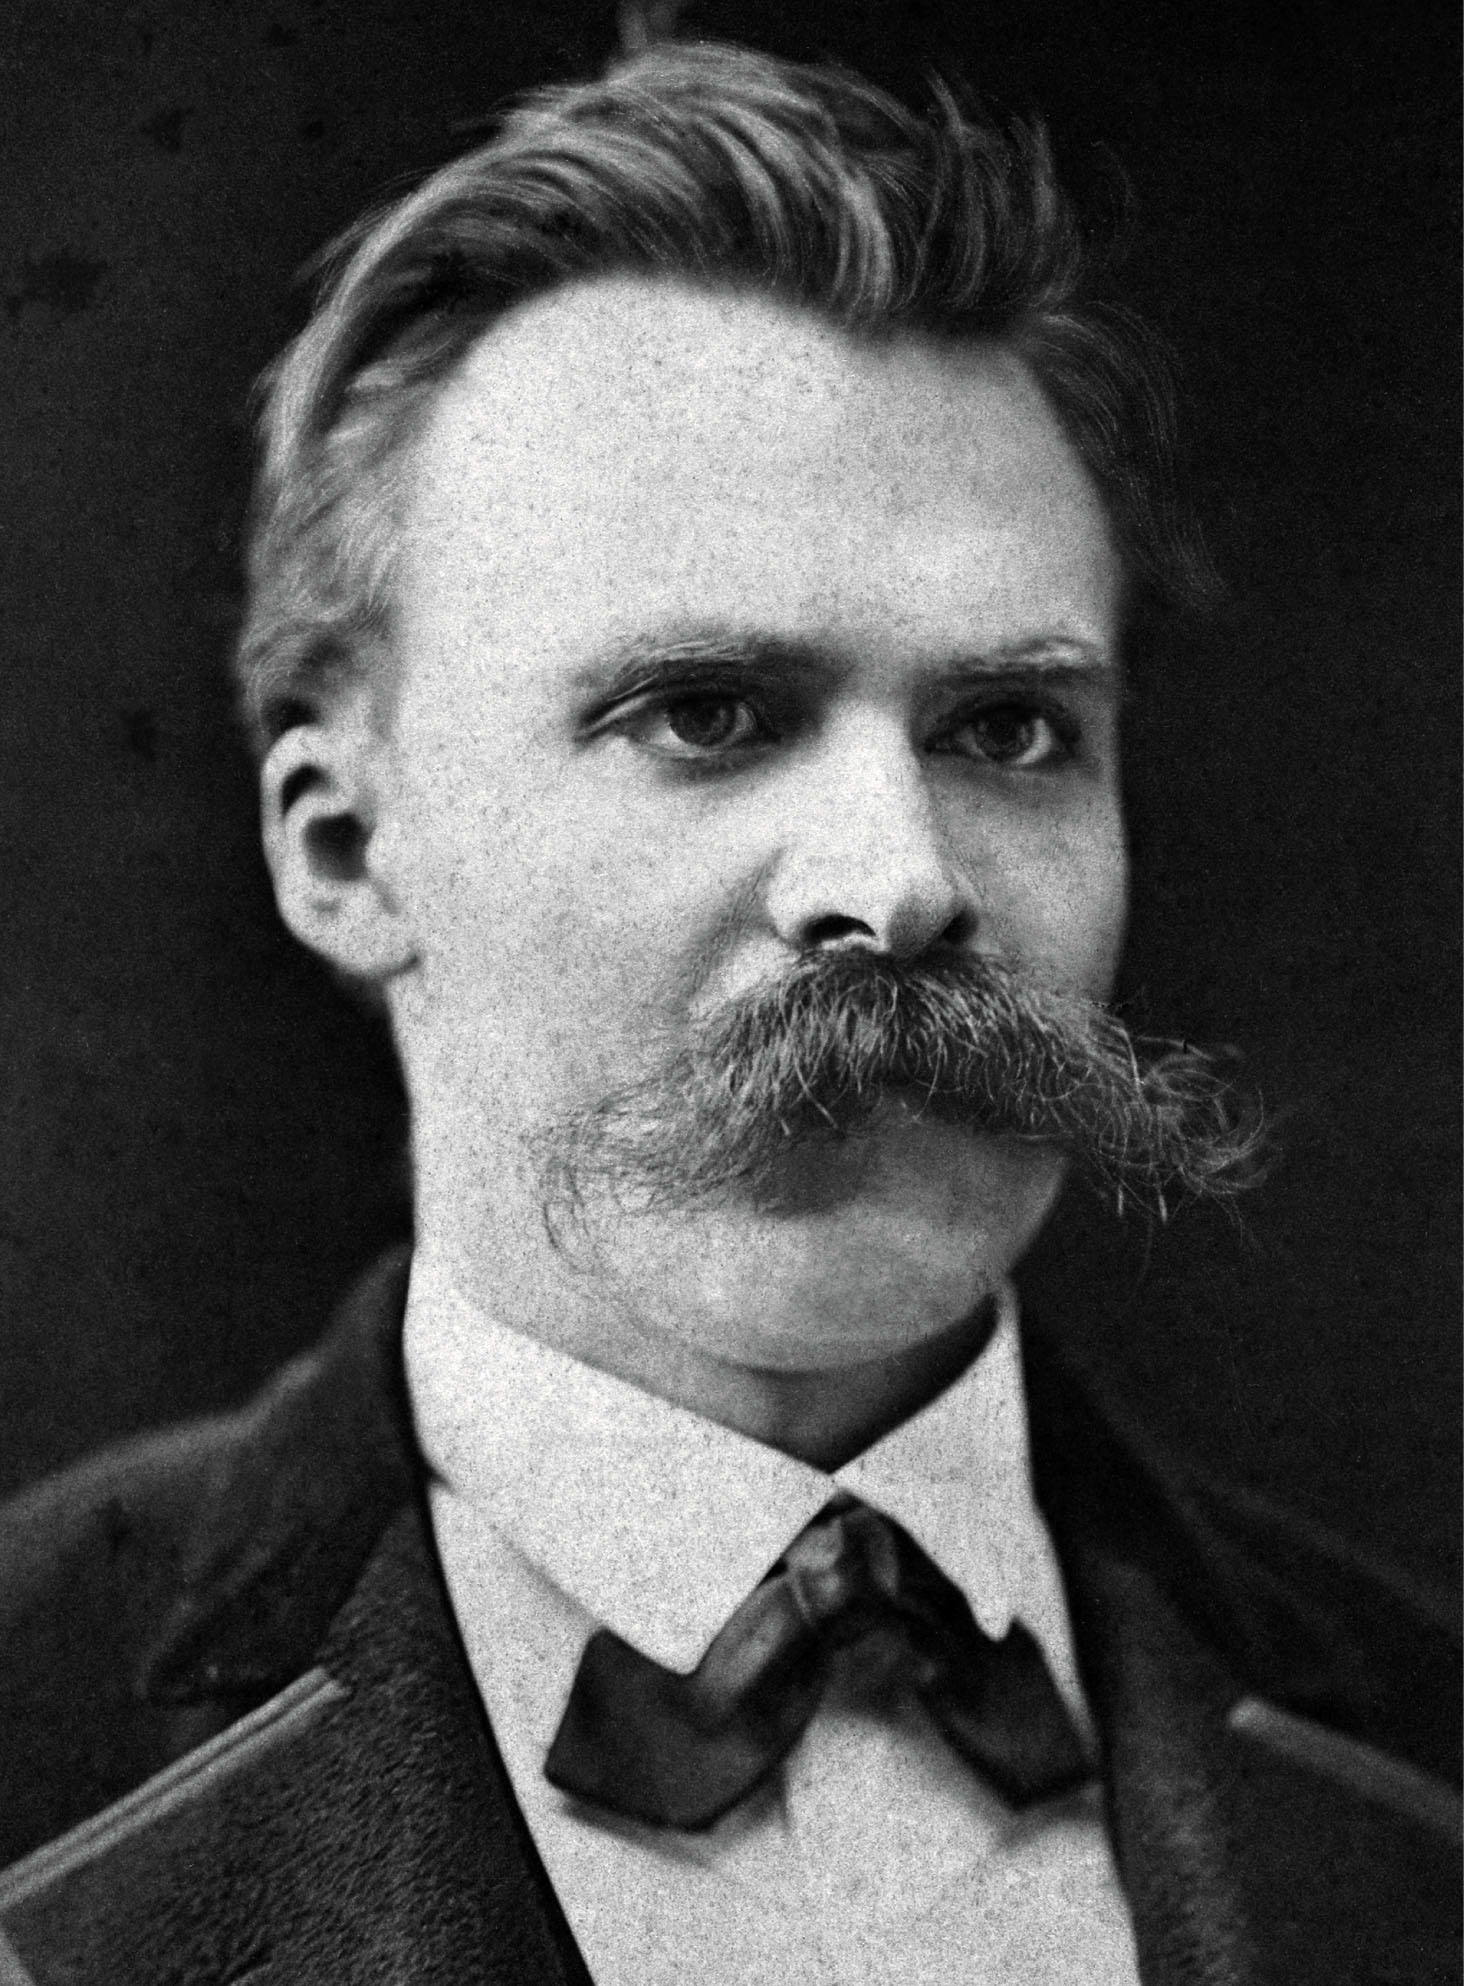
\includegraphics[width=0.7\linewidth]{Nietzsche/Nietzsche187a}\\ ``Il più abissale dei miei pensieri''}{Friedrich Nietzsche}
		Uno dei pensieri più profondi e decisivi della filosofia nietzschiana è la teoria dell'eterno ritorno dell'uguale, ovvero della ripetizione eterna di tutte le vicende del mondo, che lo stesso Nietzsche definisce ``il più abissale dei miei pensieri''. In una pagina di \textit{Ecce Homo} il filosofo afferma di essere stato folgorato da tale idea durante una passeggiata in Alta Engadina, un giorno dell'agosto 1881.\\
		Nietzsche, con la teoria dell'eterno ritorno, recupera una concezione precristiana del mondo, presente nella Grecia presocratica e nelle antiche civiltà indiane, in cui vi è una visione ciclica del tempo, opposta a quella rettilinea di tipo cristiano-moderna.
		\begin{quotation}
			``Tutto va, tutto torna indietro; eternamente ruota la ruota dell'essere. Tutto muove, tutto torna a fiorire, eternamente corre l'anno dell'essere. Tutto crolla, tutto viene di nuovo connesso; eternamente l'essere si costruisce la medesima abitazione. Tutto si diparte, tutto torna a salutarsi; eternamente fedele a se stesso rimane l'anello dell'essere. In ogni attimo comincia l'essere; attorno ad ogni "qui" ruota la sfera del "là". Il centro è dappertutto. Ricurvo è il sentiero dell'eternità.''
		\end{quotation}
		La prima formulazione della dottrina dell'eterno ritorno si incontra nell'aforisma 341 della \textit{Gaia Scienza}:
		\begin{quotation}
			 ``Che accadrebbe se, un giorno o una notte, un demone strisciasse furtivo nella più solitaria delle tue solitudini e ti dicesse: ‘Questa vita, come tu ora la vivi e l’hai vissuta, dovrai viverla ancora una volta e ancora innumerevoli volte, e non ci sarà in essa mai niente di nuovo, ma ogni dolore e ogni piacere e ogni pensiero e sospiro, e ogni indicibilmente piccola e grande cosa della tua vita dovrà fare ritorno a te, e tutte nella stessa sequenza e successione – e così pure questo ragno e questo lume di luna tra i rami e così pure questo attimo e io stesso. L’eterna clessidra dell’esistenza viene sempre di nuovo capovolta e tu con essa, granello di polvere!’ ? Non ti rovesceresti a terra, digrignando i denti e maledicendo il demone che così ha parlato? Oppure hai forse vissuto una volta un attimo immenso, in cui questa sarebbe stata la tua risposta: ‘Tu sei un dio e mai intesi cosa più divina!’? Se quel pensiero ti prendesse in suo potere, a te, quale sei ora, farebbe subire una metamorfosi, e forse ti stritolerebbe; la domanda per qualsiasi cosa ‘Vuoi tu questo ancora una volta e ancora innumerevoli volte?’ graverebbe sul tuo agire come il peso più grande! Oppure, quanto dovresti amare te stesso e la vita per non desiderare più alcun’altra cosa che questa ultima eterna sanzione, questo suggello?''
		\end{quotation}
		Già da tale passo l'eterno ritorno funge da spartiacque tra l'uomo e il superuomo: mentre il primo prova una reazione di terrore di fronte alla prospettiva dell'eterno ripetersi dell'uguale, il superuomo prova un'enorme gioia, simbolo della sua totale accettazione della vita.\\
		Un'altra interessante formulazione della teoria si trova nel discorso \textit{La visione e l'enigma} in \textit{Così parlò Zarathustra}:
		\begin{quotation}
			``Vidi un giovane pastore rotolarsi, soffocato, convulso, stravolto in viso, cui un greve serpente nero penzolava dalla bocca.
			Avevo mai visto tanto schifo e livido raccapriccio dipinto su di un volto? Forse, mentre dormiva, il serpente gli era strisciato dentro le fauci e - lì si era abbarbicato mordendo.
			La mia mano tirò con forza il serpente, tirava e tirava - invano! non riusciva a strappare il serpente dalle fauci. Allora un grido mi sfuggì dalla bocca: "Mordi! Mordi! Staccagli il capo! Mordi!", così gridò da dentro di me: il mio orrore, il mio odio, il mio schifo, la mia pietà, tutto quanto in me - buono o cattivo - gridava da dentro di me, fuso in un sol grido.-
			Voi, uomini arditi che mi circondate! Voi, dediti alla ricerca e al tentativo, e chiunque tra di voi si sia mai imbarcato con vele ingegnose per mari inesplorati! Voi che amate gli enigmi!
			Sciogliete dunque l'enigma che io allora contemplai, interpretatemi la visione del più solitario tra gli uomini!
			Giacché era una visione e una previsione: - che cosa vidi allora per similitudine? E chi è colui che un giorno non potrà non venire?
			Chi è il pastore, cui il serprente strisciò in tal modo entro le fauci? Chi è l'uomo, cui le più grevi e le più nere fra le cose strisceranno nelle fauci?
			- Il pastore, poi, morse così come gli consigliava il mio grido: e morse bene! Lontano da sé sputò la testa del serpente -; e balzò in piedi.-
			Non più pastore, non più uomo, - un trasformato, un circonfuso di luce, che rideva! Mai prima al mondo aveva riso un uomo, come lui rise!''
		\end{quotation}
		Il pastore rappresenta l'uomo in generale, il quale può trasformarsi in una creatura superiore e ridente, il superuomo, solo a patto di vincere la ripugnanza soffocante del pensiero dell'eterno ritorno (il serpente, emblema del circolo) e di prendere una coraggiosa decisione nei suoi confronti.\\
		La teoria dell'eterno ritorno rappresenta il problema oggettivamente più complesso della storiografia nietzschiana, a causa delle varie interpretazioni che si possono dare ad esso:
		\begin{itemize}
			\item potrebbe trattarsi di una \textbf{certezza cosmologica}, come talvolta afferma Nietzsche stesso, dal momento che la quantità di energia nell'universo è finita e il tempo infinito e quindi le manifestazioni e le combinazioni del mondo sono prima o poi destinate a ripetersi
			\item potrebbe invece essere un'\textbf{ipotesi sull'essere} che funge da imperativo categorico, che prescrive di amare la vita e agire come se tutto dovesse ritornare
			\item oppure potrebbe essere l'\textbf{enunciazione metaforica di un modo di essere dell'essere}, che l'uomo può incarnare solo nella misura in cui accetta la vita.
		\end{itemize}
		In ogni caso la concezione ciclica del tempo, e il conseguente rifiuto della linearità di esso, implica:
		\begin{itemize}
			\item ritenere che il \textbf{senso dell'essere} non stia fuori di esso, in un ``oltre'' irraggiungibile, ma nell'essere stesso
			\item disporsi a vivere la vita, e ogni suo attimo, come \textbf{coincidenza di essere e di senso}, realizzando così la felicità
		\end{itemize}
		Secondo Nietzsche, mentre la classica concezione lineare del tempo implica un costante tendere verso qualcosa d'altro, verso il futuro, presupponendo così l'impossibilità della felicità, la concezione ciclica restituisce ad ogni attimo il suo valore, indipendentemente dall'attimo futuro, rendendo così possibile la felicità.
		
		
		\begin{comment}
			\newpage
			\nocite{*}
			\printbibliography[heading=subbibliography, title={Testi}, type=book]
			\bigskip
			\printbibliography[heading=subbibliography, title={Siti}, keyword={sito}]
		\end{comment}

		\newpage
		\chapter{Fonti usate}
			\section{Testi}
				\begin{enumerate}[label={[\arabic*]}]
					\item Michael F. Barnsley, \textit{Fractals Everywhere}, Morgann Kaufmann Pub, Massachusetts 1993.
					\item Robert L. Devaney, \textit{Caos e frattali. Matematica dei sistemi dinamici e applicazioni al calcolatore}, Pearson Italia, Milano 2000.
					\item N. Abbagnano e G. Fornero, \textit{L'ideale e il reale. Da Schopenhauer agli sviluppi più recenti}, vol. 3 pp. 303-306, Pearson Italia, Milano 2013.
					\item Benoît B. Mandelbrot, \textit{Gli oggetti frattali}, Einaudi, Torino 2000.
				\end{enumerate}
			\section{Siti}
				\begin{enumerate}[label={[\arabic*]}]
					\item J. Cole, \textit{Finnegans Wake: Book I, Chapters 1-4}, 
					\begin{small}
						URL:
					\end{small} \texttt{http://armchairc.blogspot.it/2012/03/finnegans-wake-book-i-chapters-1-4.html}.
					\item Alison Flood, \textit{Scientists find evidence of mathematical structures in classic books}, in ``The Guardian'' (27/01/2016), 
					\begin{small}
						URL:
					\end{small}
					 \texttt{https://www.theguardian.com/books/2016/jan/27/scientists-reveal-multifractal-structure-of-finnegans-wake-james-joyce}.

					\item Tovo Flores, \textit{Nietzsche e l'eterno ritorno dell'uguale},
					\begin{small}
						URL:
					\end{small}
					\texttt{http://www.ereticamente.net/2015/12/nietzsche-e-leterno-ritorno-delluguale-tovo-flores.html}.
					\item Laura Lotti, \textit{Un'introduzione alle trasformazioni affini e ai frattali},
					\begin{small}
						URL:
					\end{small}
					\texttt{http://www.frattali.it/}.
					\item A. Strumia, \textit{Che cosa sono e a che cosa servono i frattali?}, Università di Bari, \\
					\begin{small}
						URL:
					\end{small}
					\texttt{http://www.albertostrumia.it/articoli/didattica/diart002.pdf}.
				\end{enumerate}
\end{document}